% =====================================================================
%  TP PLL – Compléments : corrections des parties B/C et parties D, E, F
%  Les figures sont dans le dossier screens/ (captures LTspice).
%  Ce fichier compile seul ; pour l'intégrer à votre Overleaf, copiez
%  uniquement ce qui se trouve entre \begin{document} et \end{document}
%  à la place des sections correspondantes, et ajoutez le dossier screens/.
% =====================================================================
\documentclass[11pt,a4paper]{article}
\usepackage[utf8]{inputenc}
\usepackage[T1]{fontenc}
\usepackage[french]{babel}
\usepackage{amsmath}
\usepackage{graphicx}
\usepackage{booktabs}
\usepackage{float}
\usepackage[margin=2.2cm]{geometry}
\graphicspath{{screens/}}

\begin{document}

% ---------------------------------------------------------------------
\section*{Corrections à apporter aux parties A, B et C}

\paragraph{Niveau de sortie du XOR.}
Dans tous les schémas de PLL (\texttt{BQ*}, \texttt{CQ*}, \texttt{DQ*}, synthétiseur), la porte
XOR n'a pas de paramètre \texttt{Vhigh} : elle utilise la valeur par défaut de LTspice,
soit $V_H = 1$~V. La simulation le confirme : \texttt{Scomp} varie entre 0 et 1~V
(figure~\ref{fig:D18v}). Il faut donc remplacer $5$~V par $1$~V dans les questions 1 et 5,
et vérifier aussi la figure~8 de la partie~A. Le gain du comparateur vaut alors
\begin{equation}
  K_D = \frac{V_H}{\pi} = \frac{1}{\pi} \approx 0{,}318~\text{V/rad},
\end{equation}
et, pour le VCO réglé de 0 à 40~kHz ($K_0 = 2\pi\times 40\,000$~rad/(s$\cdot$V)) :
\begin{equation}
  K = K_0 K_D = \frac{2\pi \times 40\,000}{\pi} = 80\,000~\text{s}^{-1}.
\end{equation}
Avec $R_1 = 5$~k$\Omega$, nous avons donc $\omega_c = 20\,000$~rad/s $= K/4$. Avec
$R_1 = 50$~k$\Omega$, nous avons $\omega_c = 2\,000$~rad/s $= K/40$.

\paragraph{Limite haute de verrouillage.}
Comme \texttt{Sfiltre} ne peut pas dépasser $V_H = 1$~V, le VCO de la boucle ne peut pas
dépasser $f_{\text{mark}} = 40$~kHz. La limite haute de verrouillage observée vers
39,8~kHz (0,995~V) correspond donc à une saturation : la boucle atteint la fréquence maximale
du VCO, et non une limite dynamique.

\paragraph{Questions 9 et 12 : seuils précis.}
Nous avons relevé les seuils directement sur les données de la simulation (fichier
\texttt{.raw}). La PLL est considérée verrouillée lorsque \texttt{SmodSchmitt} et
\texttt{SvcoSchmitt} ont le même nombre de fronts sur une fenêtre glissante de 2~ms. La
fréquence d'entrée vaut $f = 40\,V_{\text{rampe}}$ (kHz).

\begin{table}[H]
\centering
\caption{Seuils de capture et de verrouillage mesurés (rampe triangulaire 0--1~V, $C_1 = 10$~nF).}
\label{tab:seuils}
\begin{tabular}{lcccc}
\toprule
 & \multicolumn{2}{c}{$R_1 = 5$~k$\Omega$} & \multicolumn{2}{c}{$R_1 = 50$~k$\Omega$}\\
Seuil & $t$ (ms) / $V$ (V) & $f$ (kHz) & $t$ (ms) / $V$ (V) & $f$ (kHz)\\
\midrule
Capture basse $f_{CB}$ (montée)      & 110,0 / 0,220 & 8,8  & 213,8 / 0,428 & 17,1 \\
Verrouillage haut $f_{VH}$ (sommet)  & 497,6 / 0,995 & 39,8 & 497,2 / 0,994 & 39,8 \\
Capture haute $f_{CH}$ (descente)    & 636,2 / 0,728 & 29,1 & 714,0 / 0,572 & 22,9 \\
Verrouillage bas $f_{VB}$ (descente) & 924,4 / 0,151 & 6,0  & 967,2 / 0,066 & 2,6 \\
\midrule
$B_c = f_{CH} - f_{CB}$ & & \textbf{20,3} & & \textbf{5,8}\\
$B_v = f_{VH} - f_{VB}$ & & \textbf{33,8} & & \textbf{37,2}\\
\bottomrule
\end{tabular}
\end{table}

Ces valeurs remplacent les tableaux 1 et 2, et les deux encadrés « Mesure restant à effectuer » de la
question 12 peuvent être supprimés. La capture haute à 50~k$\Omega$ se produit à
$t = 714$~ms, pour $V_{\text{rampe}} = 0{,}572$~V, soit $f_{CH} = 22{,}9$~kHz
(figure~\ref{fig:B12}). La valeur de 22,46~kHz relevée à 723,7~ms était prise après la capture.

\begin{figure}[H]
\centering
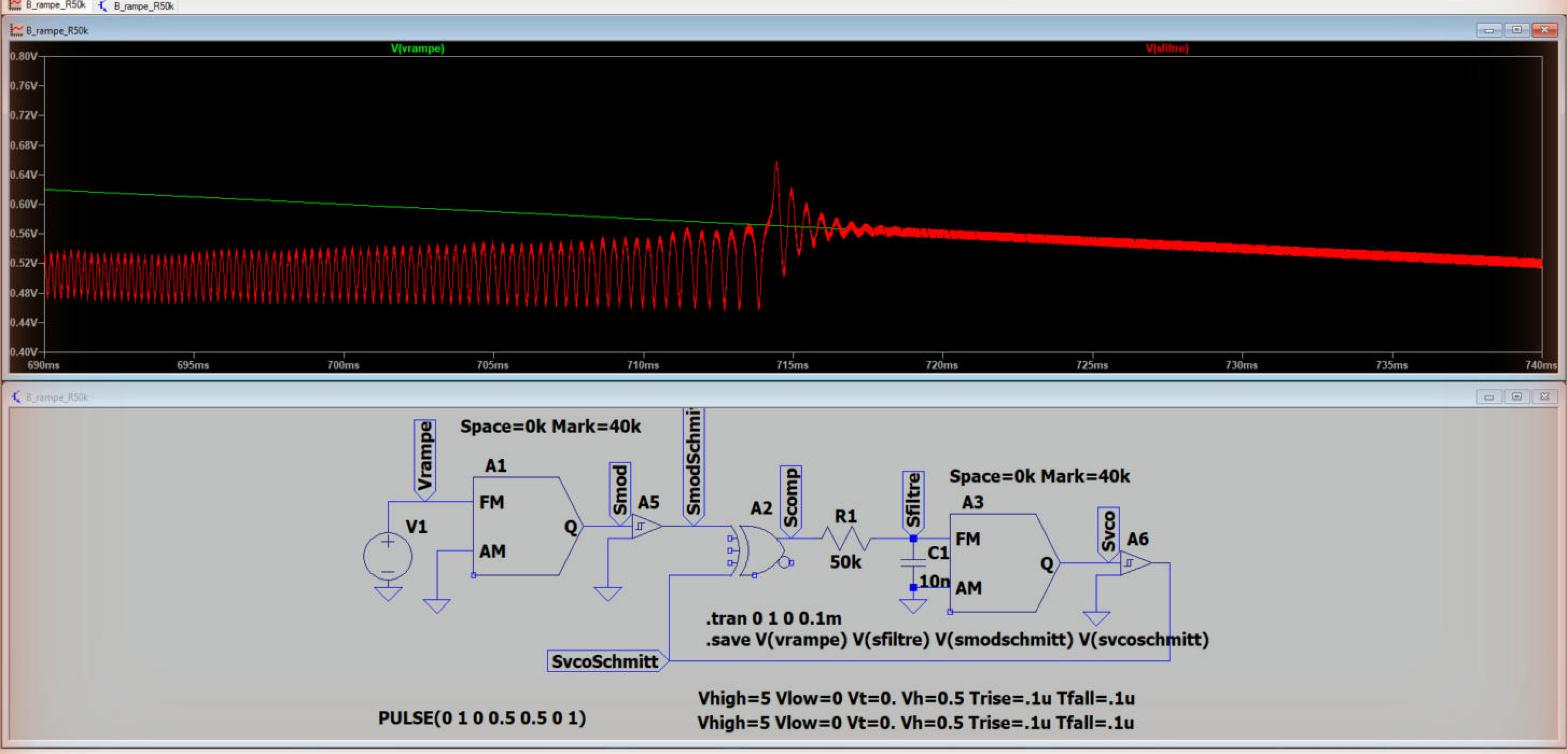
\includegraphics[width=\linewidth]{B12_capture_haute_R50k.png}
\caption{$R_1 = 50$~k$\Omega$ : capture haute pendant la descente de la rampe. Le régime
transitoire de \texttt{Sfiltre} commence à $t \approx 714$~ms, pour $V_{\text{rampe}} \approx 0{,}572$~V
(22,9~kHz).}
\label{fig:B12}
\end{figure}

Quand $R_1$ passe de 5 à 50~k$\Omega$, la bande de capture est divisée par environ 3,5
(20,3 contre 5,8~kHz). La bande de verrouillage, elle, s'élargit un peu (33,8 contre 37,2~kHz).
Le filtre étant plus sélectif, la composante de battement qui permet l'accrochage est davantage
atténuée. Une fois la boucle verrouillée, en revanche, le maintien ne dépend que de la plage
linéaire du XOR et du VCO. On retrouve l'ordre de grandeur donné par l'approximation classique
$\Delta\omega_c \approx K\,|F(j\Delta\omega_c)|$, qui donne $B_c \approx 12$~kHz pour 5~k$\Omega$
et $B_c \approx 4$~kHz pour 50~k$\Omega$. Cette approximation au premier harmonique sous-estime
toutefois les valeurs simulées.

\paragraph{Question 14 : seuils avec la sinusoïde.}
Avec \texttt{SINE(0.5 0.5 1)} et $R_1 = 50$~k$\Omega$, les mêmes mesures donnent les valeurs
du tableau~\ref{tab:sinus}. Elles remplacent le tableau~3, et l'encadré « Mesure restant à
effectuer » peut être supprimé.

\begin{table}[H]
\centering
\caption{Comparaison rampe / sinusoïde, $R_1 = 50$~k$\Omega$.}
\label{tab:sinus}
\begin{tabular}{lcccc}
\toprule
 & \multicolumn{2}{c}{Rampe} & \multicolumn{2}{c}{Sinusoïde}\\
Seuil & $V$ (V) & $f$ (kHz) & $V$ (V) & $f$ (kHz)\\
\midrule
Capture basse      & 0,428 & 17,1 & 0,426--0,429 & 17,1 \\
Capture haute      & 0,572 & 22,9 & 0,571 & 22,9 \\
Verrouillage bas   & 0,066 & 2,6  & 0,066 & 2,6 \\
Verrouillage haut  & 0,994 & 39,8 & 0,995--0,996 & 39,8 \\
\bottomrule
\end{tabular}
\end{table}

Les seuils sont identiques à la précision de la mesure : la modulation (1~Hz) est très lente
devant la dynamique de la boucle, donc la forme du signal modulant n'a pas d'influence.
Sur la sinusoïde, la boucle décroche à $t = 230$~ms (sommet), raccroche à 477~ms
(figure~\ref{fig:C14}), décroche à 668~ms (creux) et raccroche à 977~ms, puis le cycle se
répète.

\begin{figure}[H]
\centering
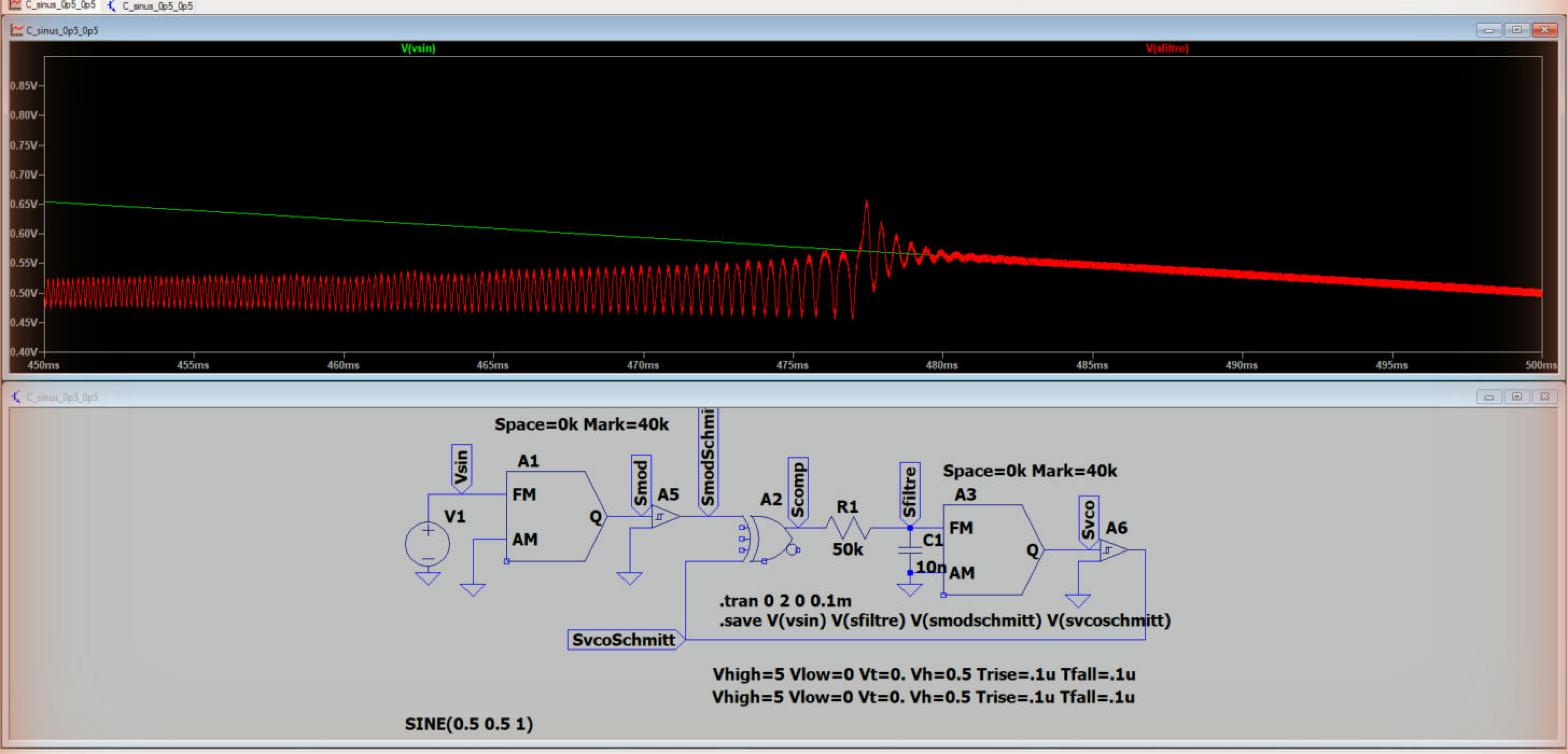
\includegraphics[width=\linewidth]{C14_capture_haute_sinus.png}
\caption{Modulation sinusoïdale \texttt{SINE(0.5 0.5 1)} : recapture à $t \approx 477$~ms,
pour $V_{\text{sin}} \approx 0{,}571$~V (22,9~kHz).}
\label{fig:C14}
\end{figure}

% ---------------------------------------------------------------------
\section{Partie D -- Démodulation d'une rampe de fréquence discrète}

\subsection{Question 16 -- Accrochage et décrochage ($R_1 = 20$~k$\Omega$)}

\begin{figure}[H]
\centering
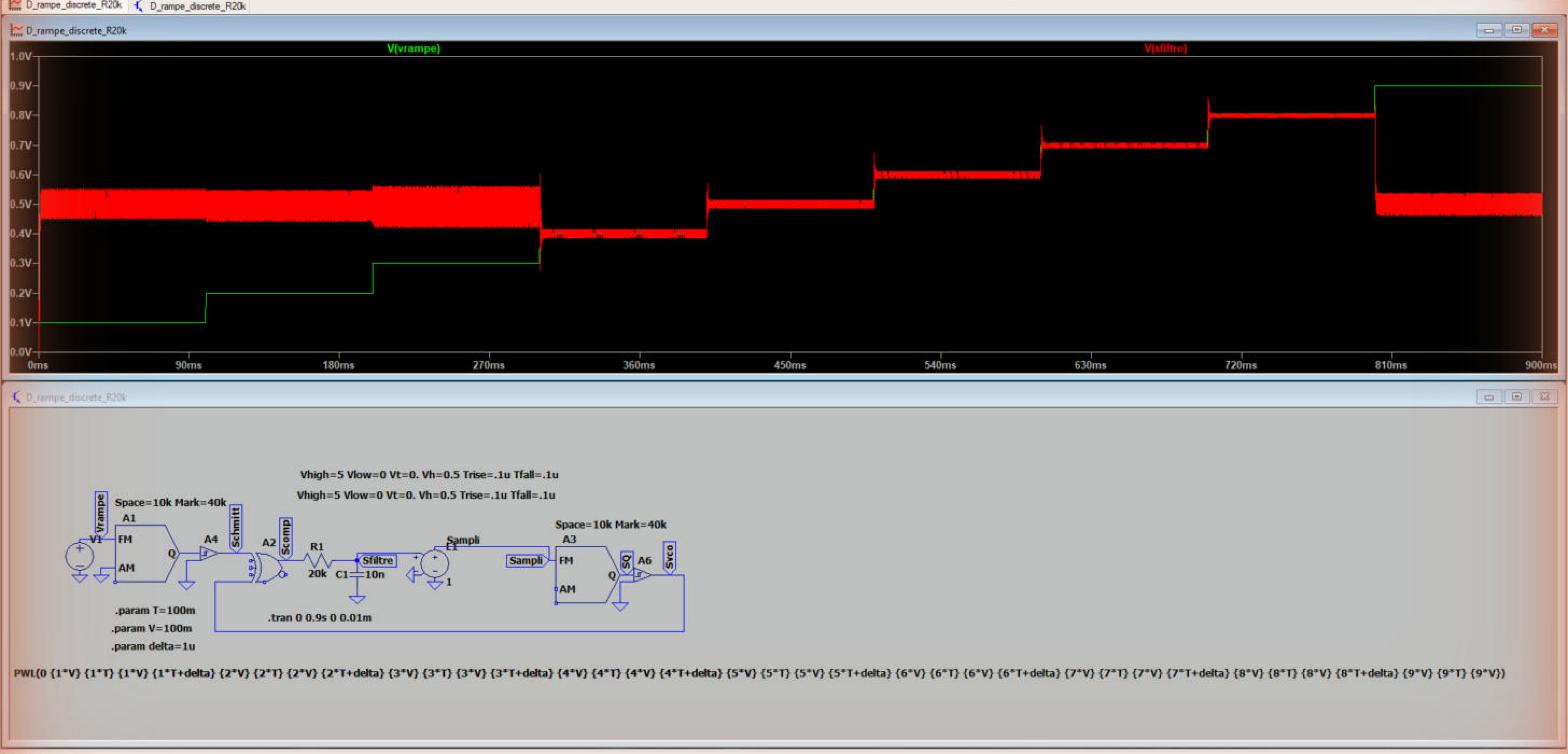
\includegraphics[width=\linewidth]{D16_rampe_discrete_R20k.png}
\caption{Rampe à paliers de 100~mV (VCO 10--40~kHz), $R_1 = 20$~k$\Omega$ : \texttt{Vrampe} (vert)
et \texttt{Sfiltre} (rouge).}
\label{fig:D16}
\end{figure}

Sur les trois premiers paliers (13, 16 et 19~kHz), \texttt{Sfiltre} reste centré sur 0,5~V
avec une forte ondulation. La boucle n'est pas verrouillée : la valeur moyenne d'un XOR
attaqué par deux signaux non synchronisés vaut $V_H/2 = 0{,}5$~V, et le VCO tourne donc à
sa fréquence libre de 25~kHz (nous mesurons 24,7 à 24,9~kHz).

\begin{itemize}
  \item \textbf{Accrochage} au saut 0,3~$\to$~0,4~V ($t = 0{,}3$~s, de 19 à 22~kHz).
  \item \textbf{Suivi} des paliers 0,4 / 0,5 / 0,6 / 0,7 / 0,8~V : la valeur moyenne de
        \texttt{Sfiltre} vaut 0,400 / 0,500 / 0,600 / 0,700 / 0,799~V et la fréquence du VCO
        est égale à celle de l'entrée (22 à 34~kHz).
  \item \textbf{Décrochage} au saut 0,8~$\to$~0,9~V ($t = 0{,}8$~s, de 34 à 37~kHz) :
        \texttt{Sfiltre} retombe à 0,5~V.
\end{itemize}

Le saut de 19 à 22~kHz réussit parce que 22~kHz se trouve dans la bande de capture autour de
25~kHz. Le saut de 34 à 37~kHz échoue : à 0,9~V, le XOR doit fonctionner avec un déphasage proche de
$0{,}9\pi$, donc près de la limite de sa zone linéaire, et le fort dépassement du transitoire (voir Q17)
fait très probablement sortir la boucle de cette zone. Une fois décrochée, la boucle ne peut pas
raccrocher à 37~kHz, qui est hors de la bande de capture.






\subsection{Question 17 -- Dépassement au saut 600~$\to$~700~mV}

\begin{figure}[H]
\centering
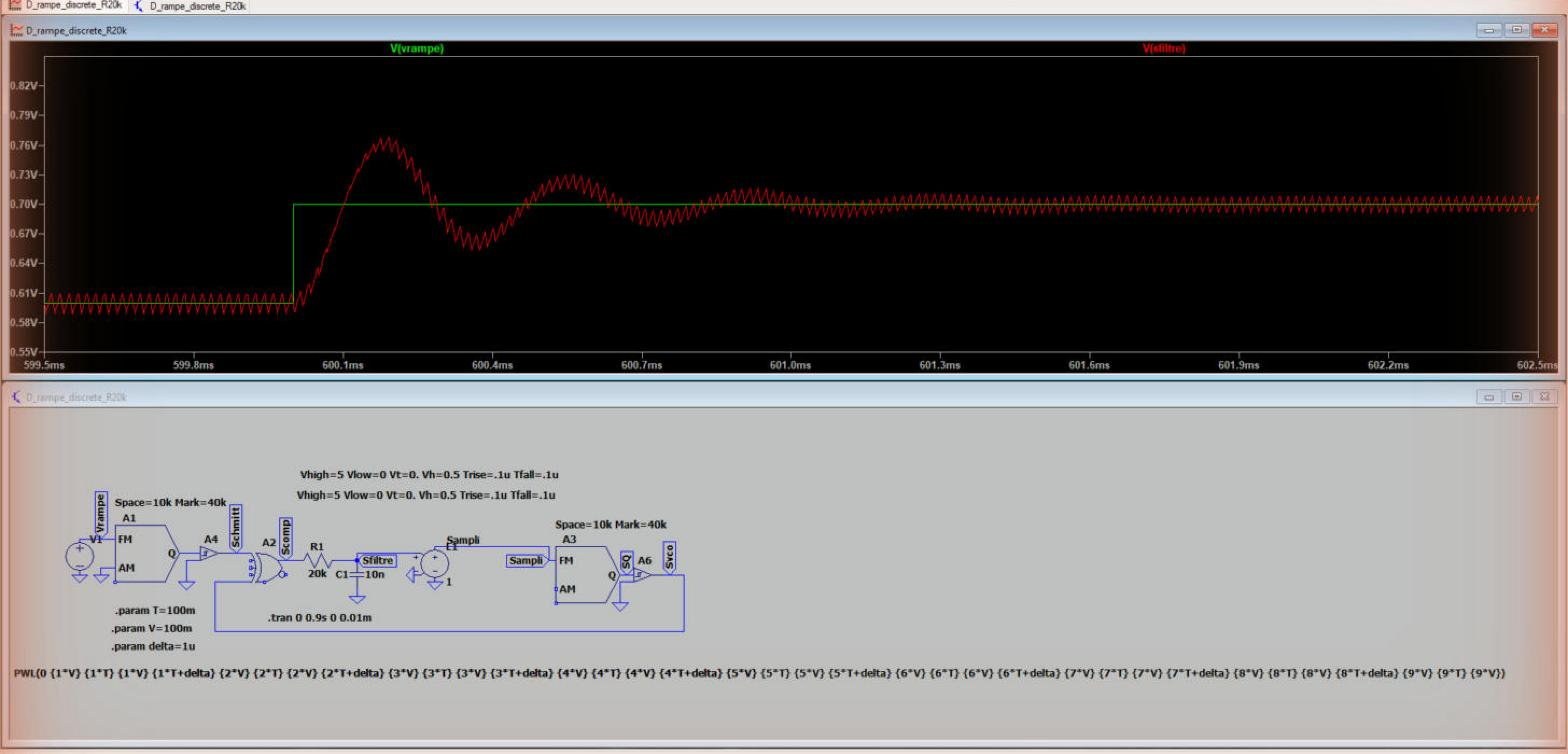
\includegraphics[width=\linewidth]{D17_saut600_700_R20k.png}
\caption{Zoom sur le saut de 600 à 700~mV ($t = 600$~ms), $R_1 = 20$~k$\Omega$.}
\label{fig:D17}
\end{figure}

Nous relevons $V_{\max} = 0{,}768$~V à $t = 600{,}19$~ms, pour une valeur finale de
$V_{\text{final}} = 0{,}700$~V :
\begin{equation}
  \Delta V_{\text{dep}} = 0{,}768 - 0{,}700 = 68~\text{mV}, \qquad
  D\% = 100 \times \frac{68}{100} \approx 68~\% .
\end{equation}
Cette valeur inclut l'ondulation résiduelle ($\pm 9$~mV). Sur la valeur moyenne de
\texttt{Sfiltre}, le dépassement vaut environ 55 à 60~\%. La réponse est oscillante amortie,
avec une pseudo-période d'environ 0,36~ms. Elle reste dans $\pm 10$~mV de la valeur finale
au bout d'environ 0,8~ms.

Ce comportement correspond à celui d'une boucle du second ordre :
\begin{equation}
  \omega_n = \sqrt{K\,\omega_c}, \qquad \zeta = \frac{1}{2}\sqrt{\frac{\omega_c}{K}} .
\end{equation}
Pour $R_1 = 20$~k$\Omega$, nous avons $\omega_c = 5\,000$~rad/s, d'où
$\omega_n = 17\,300$~rad/s, $\zeta = 0{,}14$, un dépassement théorique de
$e^{-\pi\zeta/\sqrt{1-\zeta^2}} \approx 63~\%$ et une pseudo-période de $2\pi/\omega_d \approx 0{,}37$~ms.
Ces valeurs sont cohérentes avec la simulation. Ce fort dépassement aide à comprendre le décrochage de la question 16 : au saut 0,8~$\to$~0,9~V,
le transitoire pousse le comparateur au-delà de sa zone linéaire, et la boucle perd le verrouillage.

\subsection{Question 18 -- Signaux du comparateur}

\begin{figure}[H]
\centering
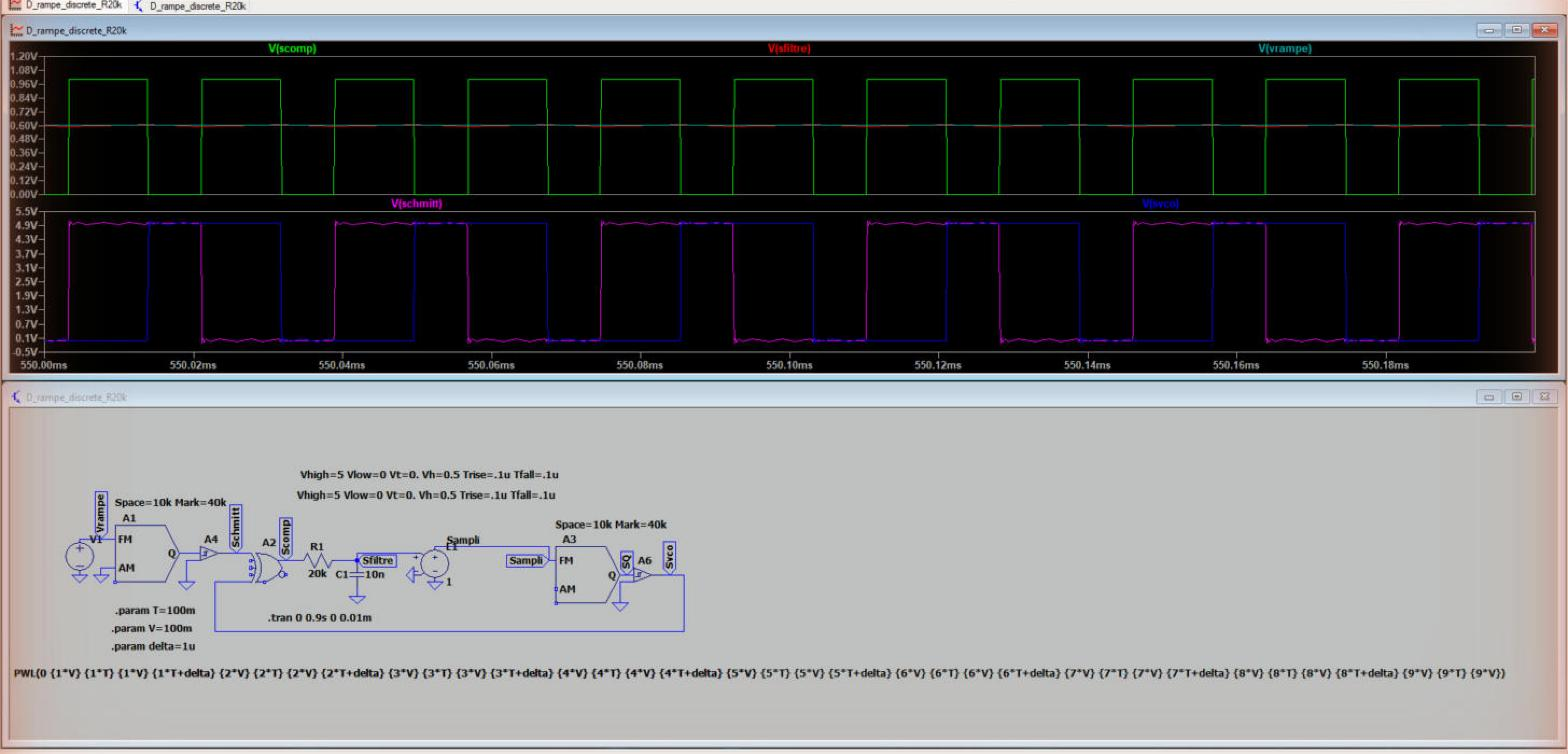
\includegraphics[width=\linewidth]{D18_verrouille_R20k.png}
\caption{Zone verrouillée ($t = 550$~ms, palier 0,6~V soit 28~kHz) : en bas \texttt{Schmitt}
(entrée) et \texttt{Svco} ; en haut \texttt{Scomp}, \texttt{Sfiltre} et \texttt{Vrampe}.}
\label{fig:D18v}
\end{figure}

\begin{figure}[H]
\centering
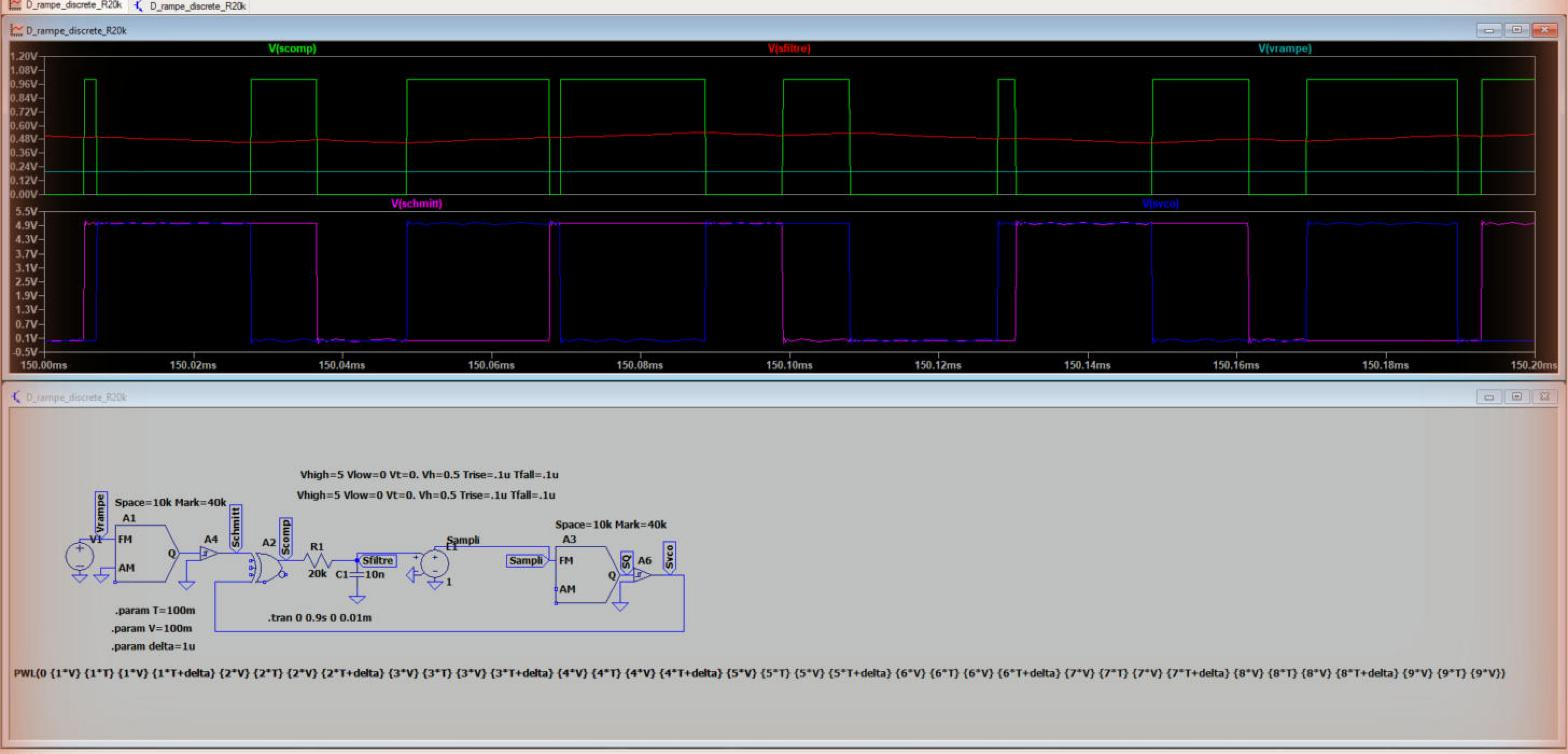
\includegraphics[width=\linewidth]{D18_non_verrouille_R20k.png}
\caption{Zone non verrouillée ($t = 150$~ms, palier 0,2~V soit 16~kHz) : mêmes signaux.}
\label{fig:D18n}
\end{figure}

\textbf{Zone verrouillée} (figure~\ref{fig:D18v}) : les deux signaux logiques ont la même
période (35,7~$\mu$s, soit 28~kHz) et un décalage constant. \texttt{Scomp} est un signal
rectangulaire régulier, de rapport cyclique 0,6, dont la moyenne vaut
0,6~V $=$ \texttt{Sfiltre} $=$ \texttt{Vrampe}. Le déphasage correspondant est
$\Delta\varphi = \pi \times 0{,}6 \approx 108^\circ$.

\textbf{Zone non verrouillée} (figure~\ref{fig:D18n}) : l'entrée est à 16~kHz et le VCO à
environ 25~kHz. Les fronts glissent les uns par rapport aux autres, et les impulsions de
\texttt{Scomp} ont une largeur qui varie d'une période à l'autre. La moyenne reste voisine de
0,5~V, ce qui ne corrige pas la fréquence du VCO. \texttt{Sfiltre} présente alors un battement
à la fréquence $|f_{\text{VCO}} - f_{\text{entrée}}|$, et non une tension continue.

\subsection{Question 19 -- Influence de $R_1$}

\begin{figure}[H]
\centering
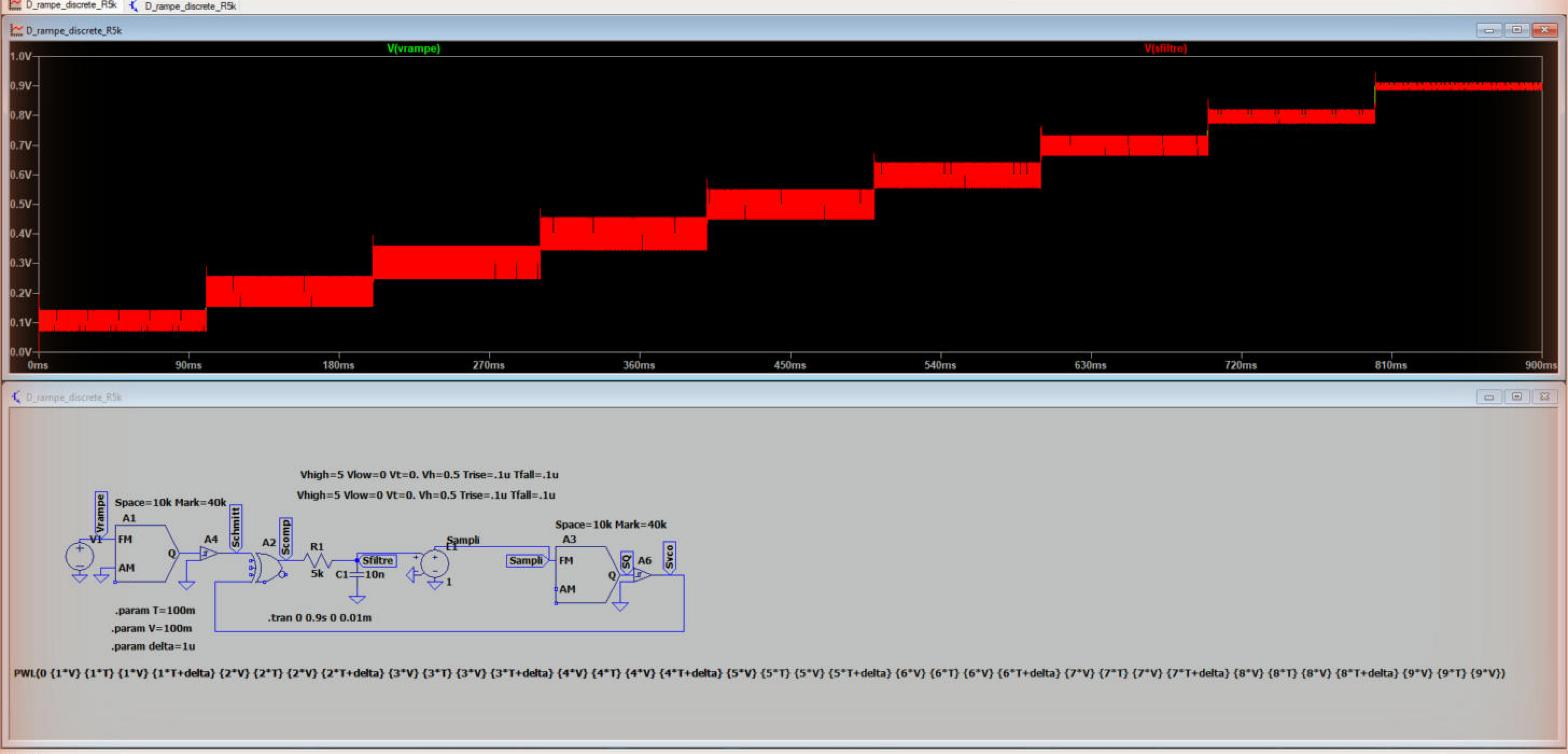
\includegraphics[width=\linewidth]{D19_R5k_full.png}
\caption{$R_1 = 5$~k$\Omega$ : tous les paliers sont suivis.}
\label{fig:D19a}
\end{figure}

\begin{figure}[H]
\centering
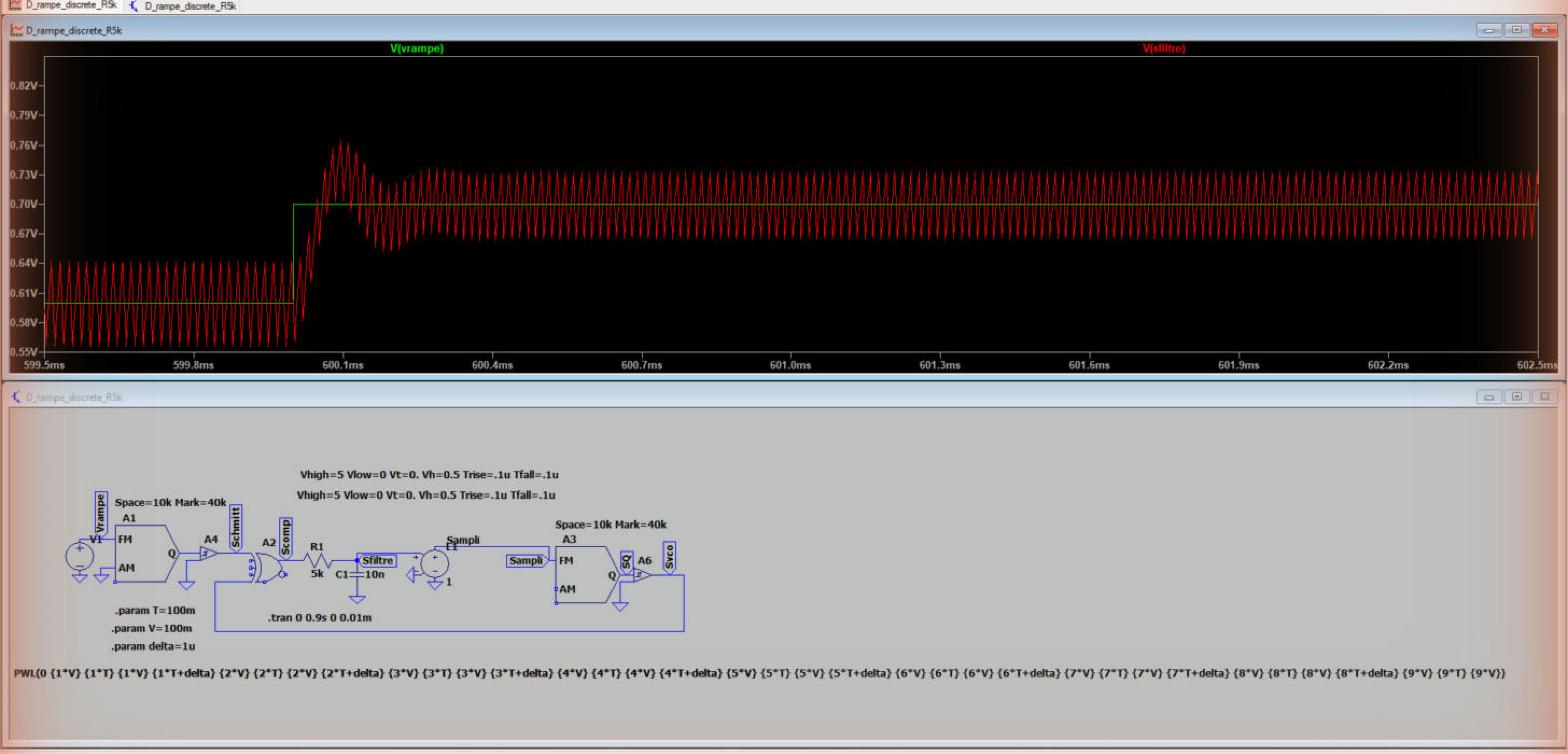
\includegraphics[width=\linewidth]{D19_R5k_saut.png}
\caption{$R_1 = 5$~k$\Omega$ : saut de 600 à 700~mV.}
\label{fig:D19b}
\end{figure}

\begin{figure}[H]
\centering
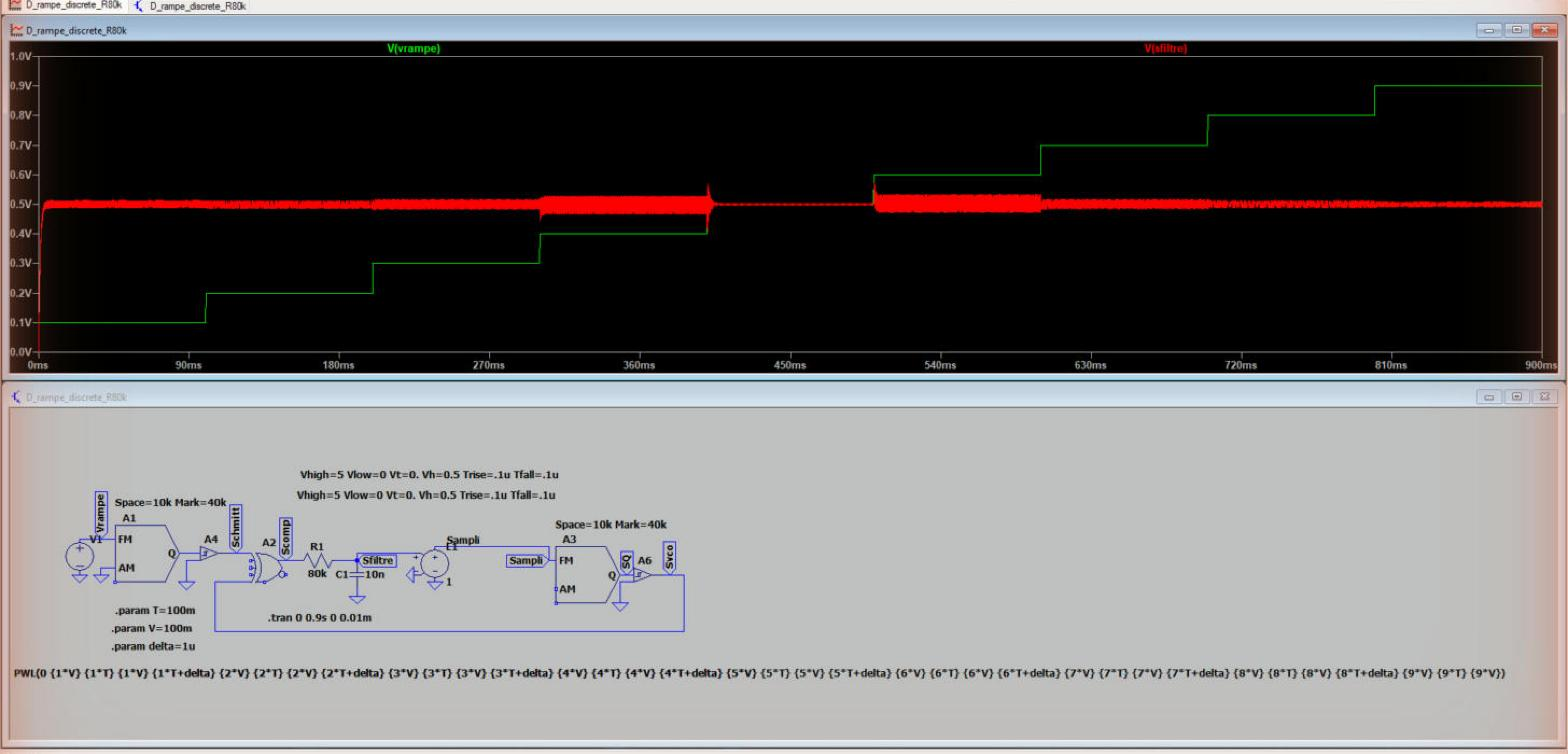
\includegraphics[width=\linewidth]{D19_R80k_full.png}
\caption{$R_1 = 80$~k$\Omega$ : la boucle ne suit pas les paliers.}
\label{fig:D19c}
\end{figure}

\begin{table}[H]
\centering
\caption{Influence de $R_1$ ($C_1 = 10$~nF, $K = 60\,000$~s$^{-1}$).}
\label{tab:R}
\begin{tabular}{lccc}
\toprule
 & 5~k$\Omega$ & 20~k$\Omega$ & 80~k$\Omega$\\
\midrule
$\tau = R_1C_1$ & 50~$\mu$s & 200~$\mu$s & 800~$\mu$s\\
$\omega_c$ (rad/s) & 20\,000 & 5\,000 & 1\,250\\
$\zeta$ théorique & 0,29 & 0,14 & 0,07\\
Dépassement théorique & 39~\% & 63~\% & 80~\%\\
Paliers suivis & tous (13--37~kHz) & 22--34~kHz & aucun\\
Ondulation de \texttt{Sfiltre} (crête à crête) & 25 à 110~mV & 12 à 28~mV & $\approx$ 6~mV\\
Dépassement mesuré (600$\to$700~mV) & 66~mV & 68~mV & --\\
Temps de réponse ($\pm10$~mV) & 0,15~ms & 0,8~ms & --\\
\bottomrule
\end{tabular}
\end{table}

\begin{itemize}
  \item \textbf{5~k$\Omega$} : la boucle est rapide et bien amortie ($\zeta \approx 0{,}3$). Elle
        suit tous les paliers et sa bande de capture est large. En contrepartie, le filtrage est
        faible : l'ondulation à $2f$ reste importante. La pointe de 66~mV est due surtout à cette
        ondulation, qui atteint déjà $\pm 40$~mV en régime établi ; le dépassement réel de la
        valeur moyenne n'est que d'environ 20~mV.
  \item \textbf{20~k$\Omega$} : c'est un compromis. L'ondulation est plus faible, mais la réponse
        est peu amortie (dépassement d'environ 60~\%) et la bande de capture est réduite.
  \item \textbf{80~k$\Omega$} : le filtrage est excellent (ondulation d'environ 6~mV), mais la bande
        de capture est trop étroite. La boucle n'est jamais capturée : \texttt{Sfiltre} reste à
        0,5~V, et le VCO à sa fréquence libre de 25~kHz. Il n'y a qu'au palier 0,5~V
        ($t = 0{,}4$ à 0,5~s) que la sortie coïncide avec l'entrée, parce que 25~kHz est
        justement la fréquence libre.
\end{itemize}
Augmenter $R_1$ améliore donc le filtrage, au détriment de la bande de capture, de
l'amortissement et de la rapidité.

% ---------------------------------------------------------------------
\section{Partie E -- Démodulation d'un signal FSK}

\subsection{Question 20 -- Saut de fréquence maximal}
Nous avons conservé le montage FSK fourni (VCO de 0 à 40~kHz, $R_1 = 50$~k$\Omega$,
$C_1 = 10$~nF, bits de 100~ms). Les deux tensions sont centrées sur 0,5~V (20~kHz) :
$V_{1,2} = 0{,}5 \mp D/2$. Un balayage \texttt{.step} a donné les résultats suivants :

\begin{table}[H]
\centering
\caption{Démodulation FSK en fonction de l'écart $D = V_2 - V_1$.}
\label{tab:fsk}
\begin{tabular}{cccc}
\toprule
$D$ (V) & $f_1$ / $f_2$ (kHz) & $\Delta f$ (kHz) & Démodulation\\
\midrule
0,05 & 19 / 21 & 2 & correcte\\
0,10 & 18 / 22 & 4 & correcte\\
0,15 & 17 / 23 & 6 & correcte (limite)\\
0,16 à 0,19 & -- & 6,4 à 7,6 & bits perdus\\
0,20 & 16 / 24 & 8 & bits perdus\\
$\geq 0{,}3$ & -- & $\geq 12$ & aucun bit restitué\\
\bottomrule
\end{tabular}
\end{table}

\begin{figure}[H]
\centering
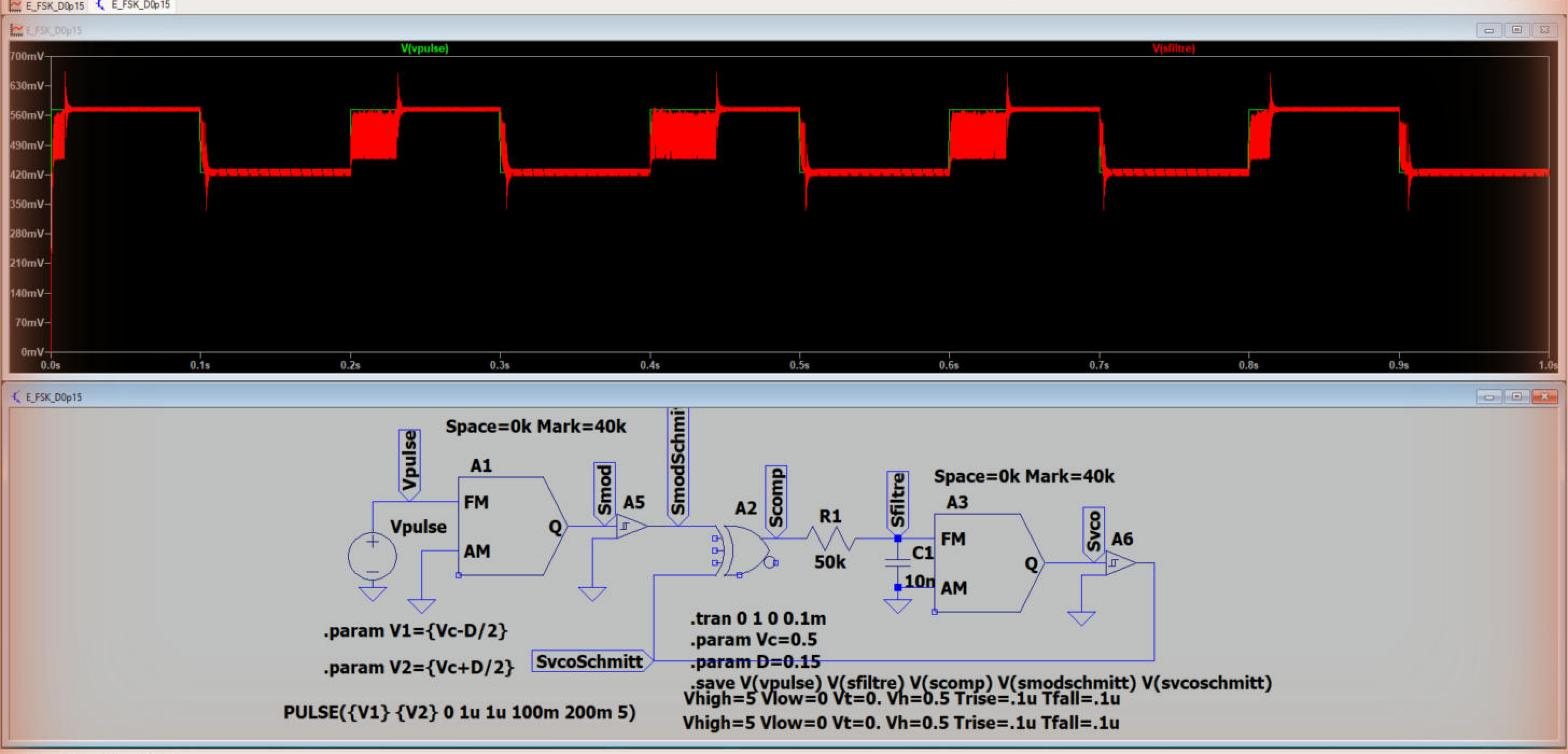
\includegraphics[width=\linewidth]{E20_FSK_D0p15_ok.png}
\caption{FSK avec $D = 0{,}15$~V (17 / 23~kHz) : \texttt{Sfiltre} restitue tous les bits.}
\label{fig:E20ok}
\end{figure}

\begin{figure}[H]
\centering
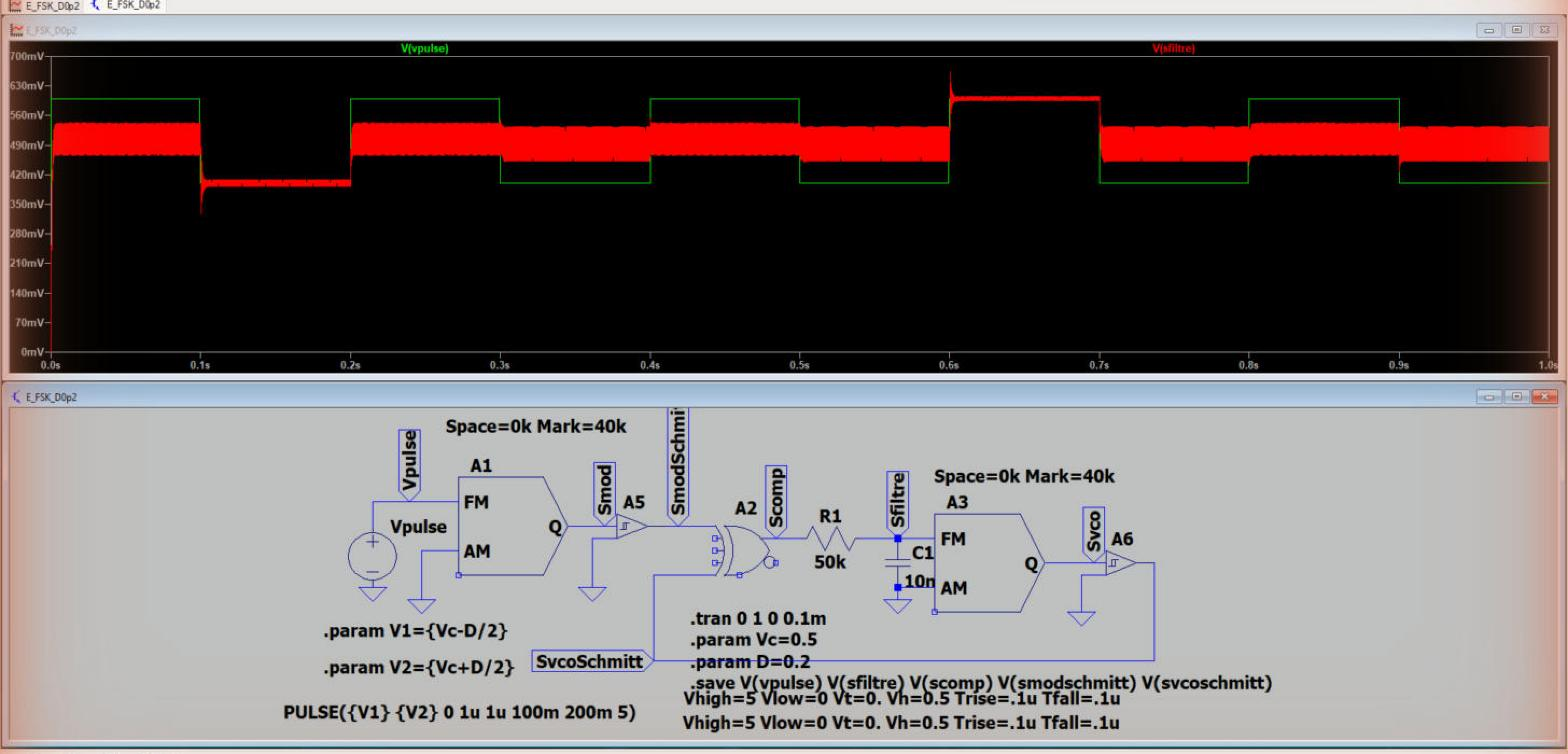
\includegraphics[width=\linewidth]{E20_FSK_D0p2_ko.png}
\caption{FSK avec $D = 0{,}2$~V (16 / 24~kHz) : la boucle reste décrochée sur la plupart des bits.}
\label{fig:E20ko}
\end{figure}

Le saut maximal correctement démodulé est donc de $\Delta f \approx 6$~kHz, entre 17 et 23~kHz.
Cette valeur correspond exactement à la bande de capture mesurée à 50~k$\Omega$
(17,1--22,9~kHz, tableau~\ref{tab:seuils}). À chaque changement de bit, le saut de fréquence
est instantané : la boucle perd la phase et doit se recapturer sur la nouvelle fréquence.
Les deux fréquences doivent donc se trouver dans la bande de capture, et pas seulement dans la
bande de verrouillage. Avec $D = 0{,}15$~V, on voit déjà, sur les bits hauts, une recapture
d'environ 30~ms (zone d'ondulation au début du bit). Au-delà, certains bits ne sont jamais
recapturés et \texttt{Sfiltre} reste à 0,5~V. Pour accepter des sauts plus grands, il faudrait
réduire $R_1$ afin d'élargir la bande de capture, au prix d'une ondulation plus forte.

% ---------------------------------------------------------------------
\section{Partie F -- Synthétiseur de fréquence}
Le montage utilise une horloge de 10~kHz, $N = 3$, un VCO de 10 à 40~kHz
(\texttt{Space=10k Mark=40k}) et un filtre de 5~k$\Omega$ et 10~nF ($\omega_c = 20\,000$~rad/s).
La sortie du compteur varie entre 0 et 1~V, et le XOR entre 0 et 1~V.

\subsection{Question 21 -- Régime transitoire}

\begin{figure}[H]
\centering
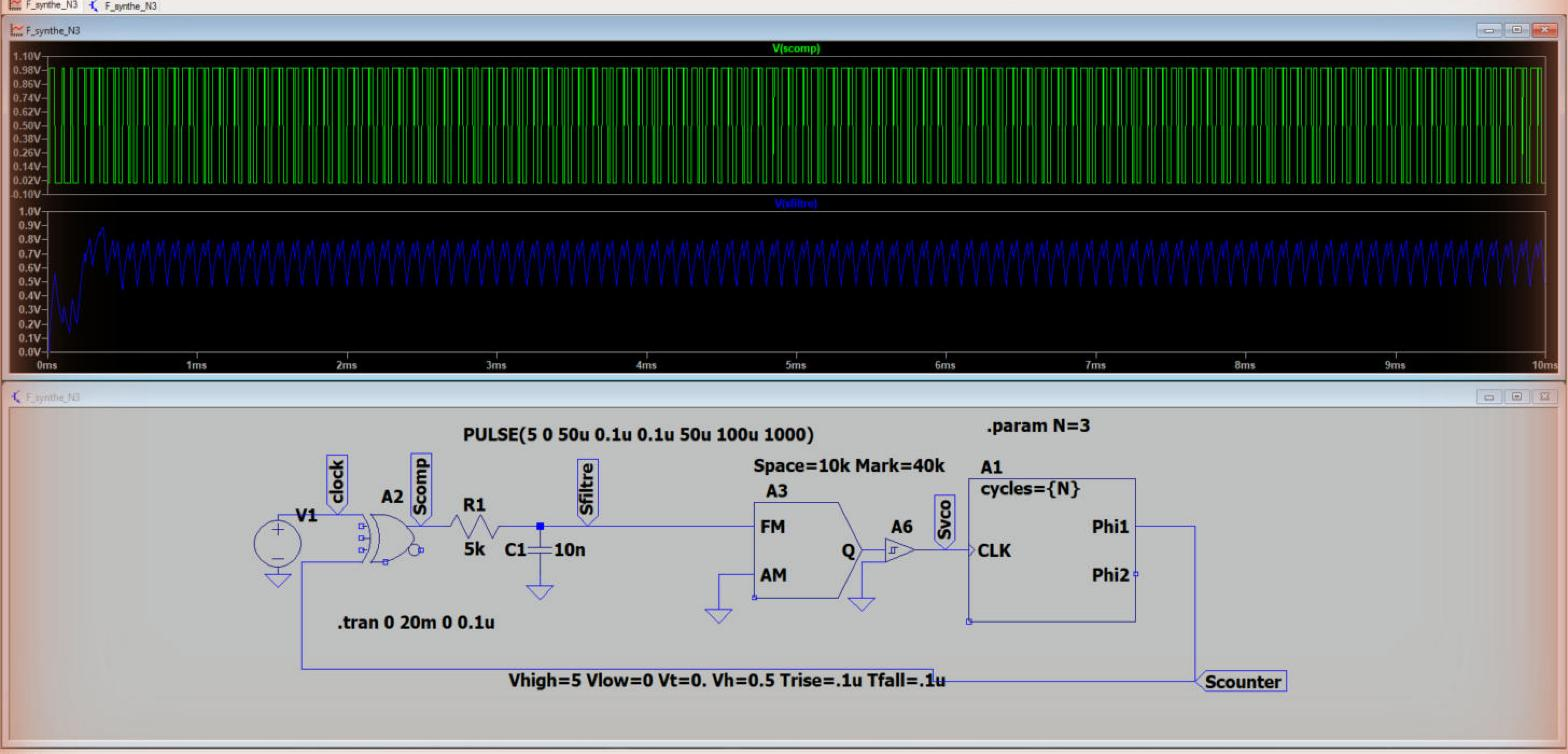
\includegraphics[width=\linewidth]{F21_transitoire_10ms.png}
\caption{\texttt{Scomp} et \texttt{Sfiltre} sur les 10 premières millisecondes.}
\label{fig:F21}
\end{figure}

\begin{figure}[H]
\centering
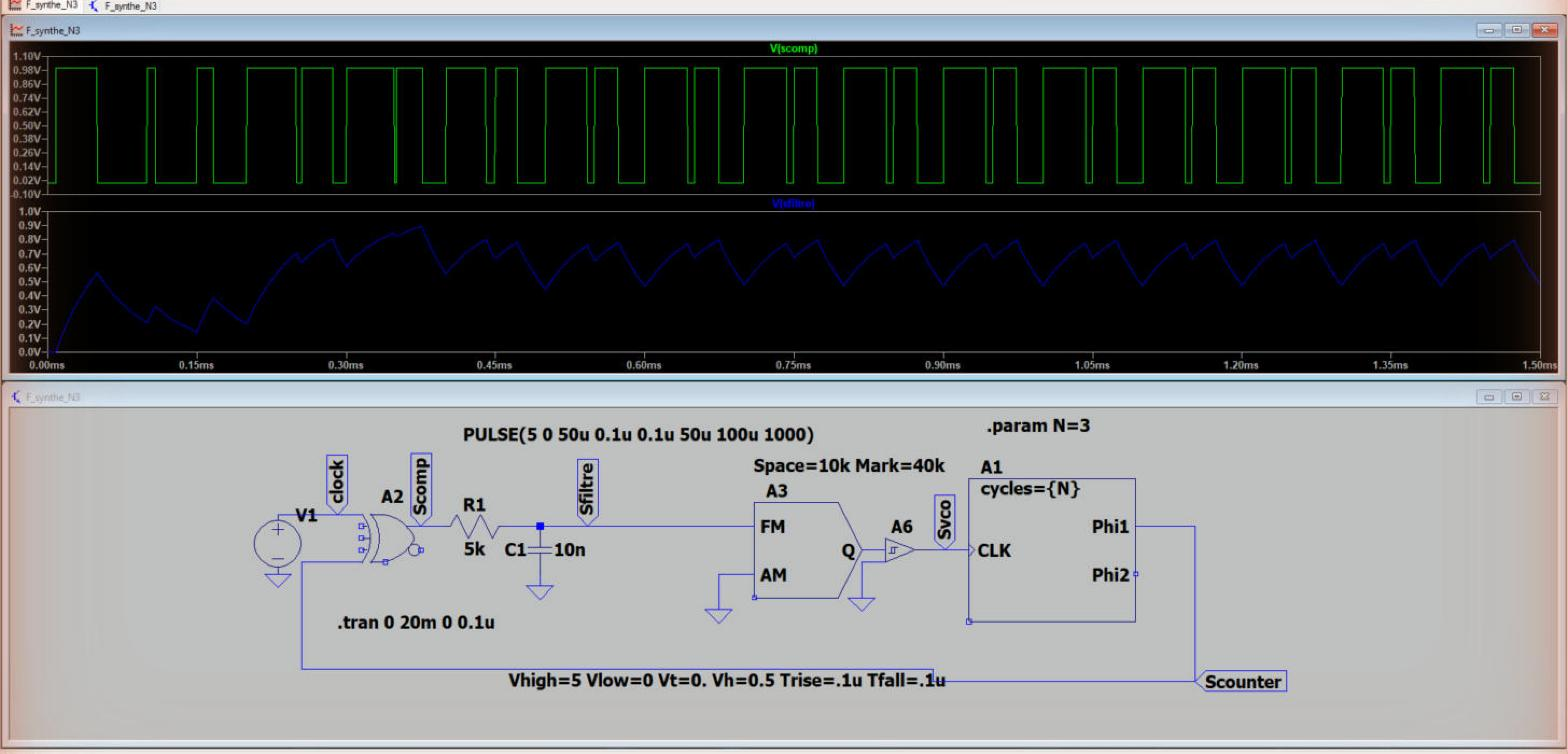
\includegraphics[width=\linewidth]{F21_transitoire_zoom.png}
\caption{Zoom sur les 1,5 premières millisecondes.}
\label{fig:F21z}
\end{figure}

Nous distinguons quatre phases (figure~\ref{fig:F21z}) :
\begin{enumerate}
  \item \textbf{0 à 0,2~ms -- acquisition} : la boucle n'est pas verrouillée. Le VCO démarre à
        environ 19~kHz, \texttt{Sfiltre} oscille entre 0,15 et 0,55~V, et \texttt{Scomp} a un
        rapport cyclique irrégulier.
  \item \textbf{0,2 à 0,38~ms -- montée} : la valeur moyenne de \texttt{Sfiltre} monte rapidement
        vers 0,67~V.
  \item \textbf{0,38 à 0,6~ms -- dépassement et oscillations amorties} : nous mesurons une pointe
        de 0,90~V à 0,38~ms (0,78~V en valeur moyenne, soit environ 0,12~V au-dessus de la valeur
        finale), puis deux à trois oscillations amorties.
  \item \textbf{Au-delà de 0,6~ms -- régime établi} : la valeur moyenne est constante, avec une
        ondulation en dents de scie entre 0,47 et 0,80~V, à la fréquence de référence.
\end{enumerate}
Avec le diviseur, le gain de boucle vaut $K = K_0K_D/N = 60\,000/3 = 20\,000$~s$^{-1}$, d'où
$\omega_n = \sqrt{K\omega_c} = 20\,000$~rad/s et $\zeta = 0{,}5$. Une réponse bien amortie, avec
peu d'oscillations, est donc attendue, ce que confirme la simulation.

\subsection{Question 22 -- Temps d'établissement et tension finale}
La valeur moyenne finale de \texttt{Sfiltre} vaut $0{,}667$~V, ce qui correspond exactement à la
valeur théorique $(30-10)/(40-10) = 0{,}667$~V. En prenant comme critère une valeur moyenne
restant dans $\pm 20$~mV de la valeur finale, le temps d'établissement vaut
\begin{equation}
  t_e \approx 0{,}58~\text{ms} \quad\Rightarrow\quad N_p = \frac{t_e}{T_{\text{ref}}} = \frac{0{,}58}{0{,}1} \approx 6~\text{périodes d'horloge}.
\end{equation}
Avec $\pm 10$~mV, nous obtenons $t_e \approx 0{,}64$~ms, soit environ 6,5 périodes.

\subsection{Question 23 -- Rapport de fréquence}

\begin{figure}[H]
\centering
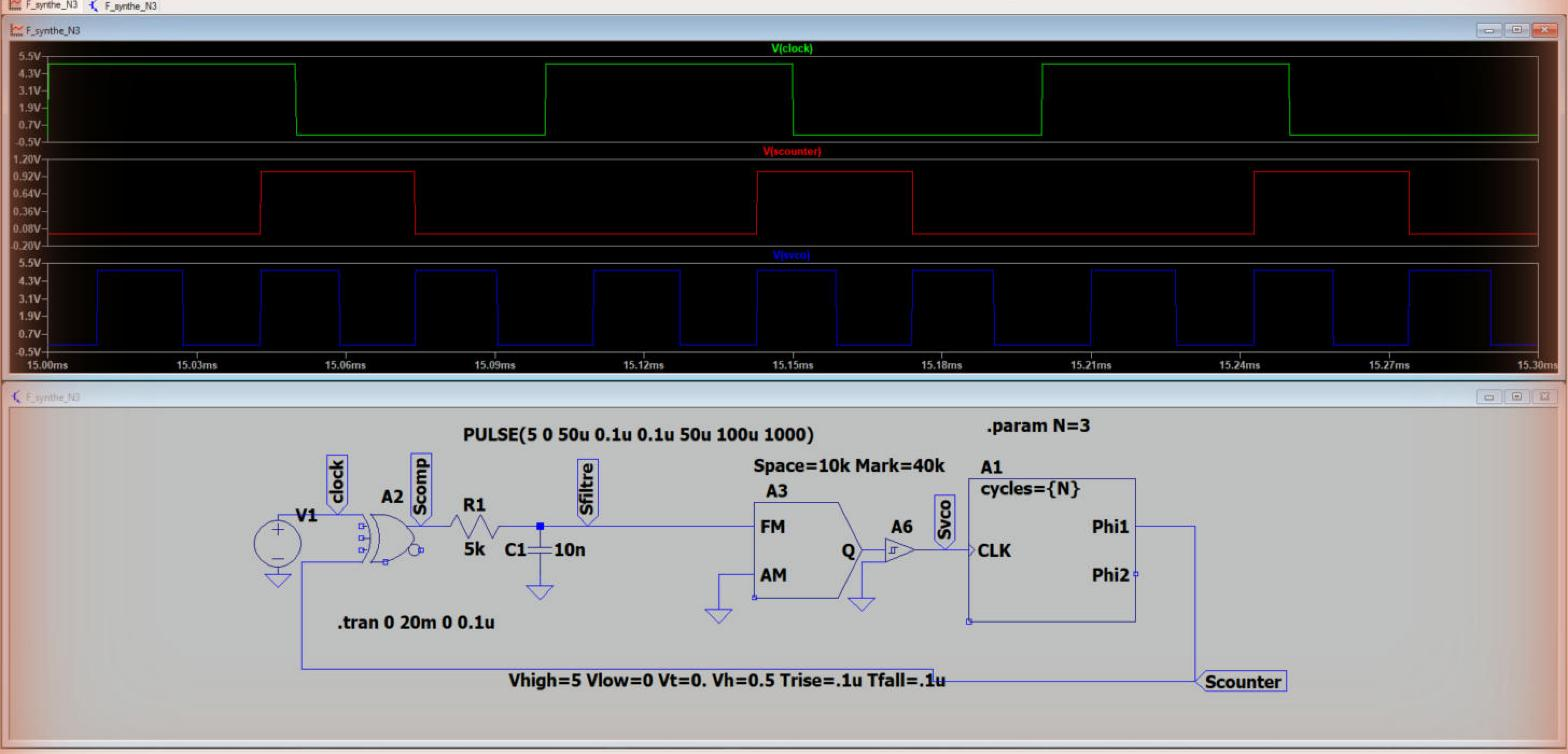
\includegraphics[width=\linewidth]{F23_clock_counter_vco.png}
\caption{Régime établi ($t = 15$~ms) : \texttt{clock}, \texttt{Scounter} et \texttt{Svco}.}
\label{fig:F23}
\end{figure}

\texttt{clock} et \texttt{Scounter} ont la même période de 100~$\mu$s (10,000~kHz), et nous
comptons exactement trois périodes de \texttt{Svco} (33,3~$\mu$s) par période d'horloge.
Sur la partie stable (6 à 20~ms), nous mesurons $f_{\text{VCO}} = 30{,}006$~kHz : le rapport
$N = 3$ est vérifié. Le signal \texttt{Scounter} a un rapport cyclique de 1/3 (il reste haut
pendant une seule période du VCO), alors que l'horloge a un rapport cyclique de 50~\%.

\subsection{Question 24 -- Analyse spectrale}

\begin{figure}[H]
\centering
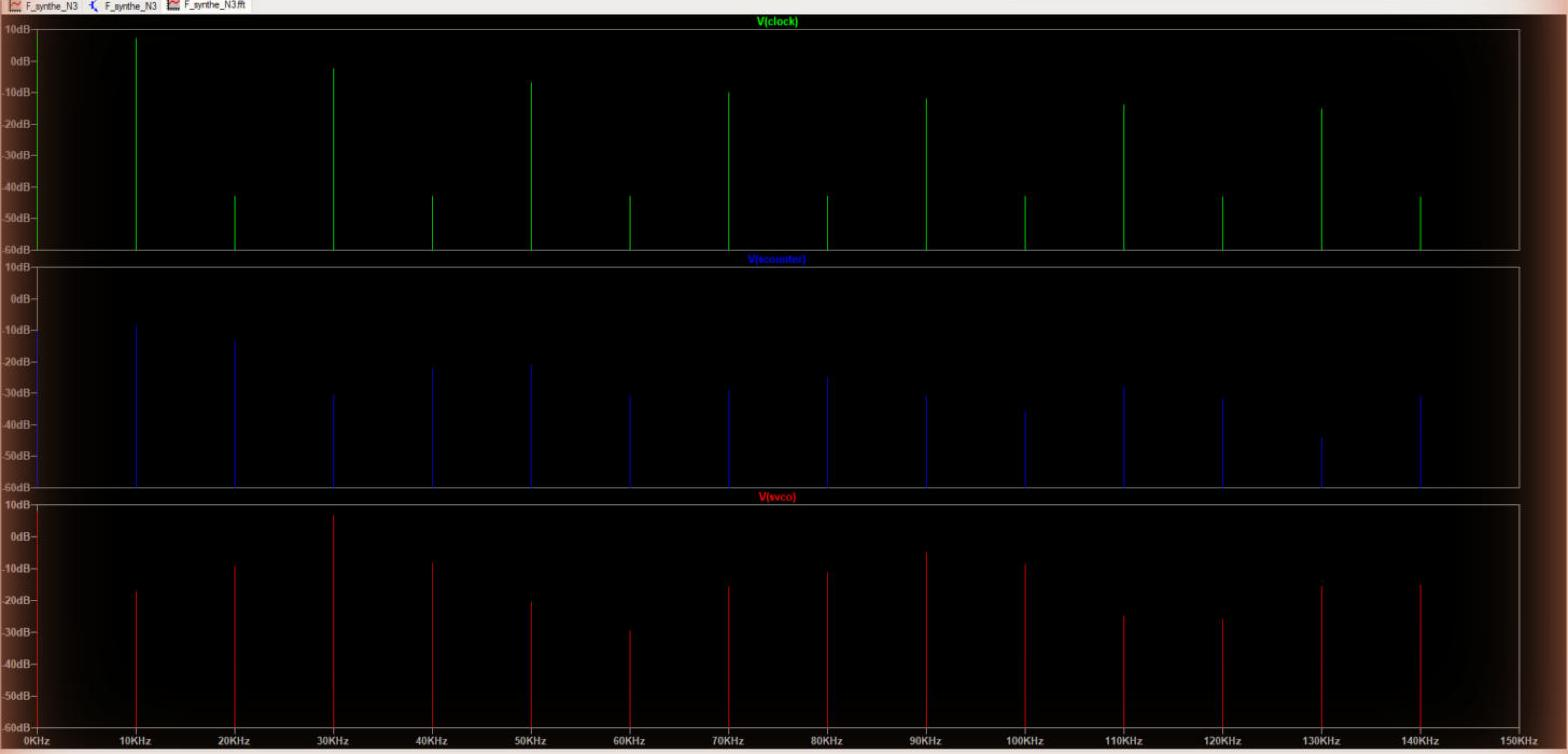
\includegraphics[width=\linewidth]{F24_FFT.png}
\caption{FFT entre 6 et 20~ms (262\,144 points, sans fenêtre) de \texttt{clock},
\texttt{Scounter} et \texttt{Svco}, de $+10$ à $-60$~dB et de 0 à 150~kHz.}
\label{fig:F24}
\end{figure}

\begin{table}[H]
\centering
\caption{Niveaux des raies (dB, valeur efficace).}
\label{tab:fft}
\begin{tabular}{lcccccc}
\toprule
 & 10~kHz & 20~kHz & 30~kHz & 40~kHz & 50~kHz & 90~kHz\\
\midrule
\texttt{clock}    & \textbf{+7,0} & $-43$ & $-2{,}5$ & $-43$ & $-6{,}9$ & $-12{,}0$\\
\texttt{Scounter} & \textbf{$-8{,}5$} & $-13{,}6$ & $-30{,}5$ & $-22{,}0$ & $-21{,}1$ & $-31{,}0$\\
\texttt{Svco}     & $-17{,}1$ & $-9{,}3$ & \textbf{+6,8} & $-8{,}5$ & $-20{,}4$ & $-4{,}9$\\
\bottomrule
\end{tabular}
\end{table}

\begin{itemize}
  \item \textbf{clock} : raie fondamentale à 10~kHz et uniquement des harmoniques impairs
        (30, 50, 70~kHz\dots) décroissant en $1/n$. C'est le spectre attendu d'un signal carré
        de rapport cyclique 50~\%.
  \item \textbf{Scounter} : fondamentale à 10~kHz, harmoniques pairs et impairs, et un creux à
        30, 60 et 90~kHz. Ce creux vient du rapport cyclique de 1/3 : l'enveloppe en sinus
        cardinal s'annule pour les multiples de 3.
  \item \textbf{Svco} : la raie principale est bien à 30~kHz (+6,8~dB). Elle est entourée de
        raies parasites à $30 \pm 10$~kHz (20 et 40~kHz), à seulement 16~dB sous la porteuse.
        Elles viennent de la forte ondulation de \texttt{Sfiltre} à 10~kHz (0,47--0,80~V), qui
        module en fréquence le VCO : sa fréquence instantanée varie entre 27,8 et 32,0~kHz
        au cours d'une période d'horloge.
\end{itemize}
Les raies sont fines : avec une résolution de $1/14~\text{ms} \approx 71$~Hz, il n'y a pas
d'élargissement visible, car le signal est parfaitement périodique en simulation (aucun bruit).
La qualité spectrale du synthétiseur est donc limitée par ces raies parasites de référence
(\emph{reference spurs}), et non par du bruit de phase aléatoire. Pour les réduire, il faudrait
un filtre plus sélectif (plus grand $R_1$ ou un filtre d'ordre supérieur) ou un comparateur
phase-fréquence, au prix d'une boucle plus lente.

\subsection{Question 25 -- Variante : diviseur par 8 à bascules D}
Nous avons réalisé le diviseur avec trois bascules D en cascade (compteur asynchrone). Pour
chaque bascule, $D$ est relié à $\overline{Q}$, ce qui la fait basculer à chaque front. Chaque
étage divise donc la fréquence par 2, et $2^3 = 8$. Comme $8 \times 10~\text{kHz} = 80$~kHz
dépasse la plage du VCO (10--40~kHz), nous avons pris une référence de 4~kHz, d'où
$f_{\text{VCO}} = 32$~kHz et $V_{\text{filtre}} = (32-10)/30 = 0{,}733$~V théoriques. Le filtre
est ici de 20~k$\Omega$ et 10~nF. La simulation a été réalisée à partir d'une netlist
(\texttt{F\_synthe\_N8\_bascules\_D.cir}).

\begin{figure}[H]
\centering
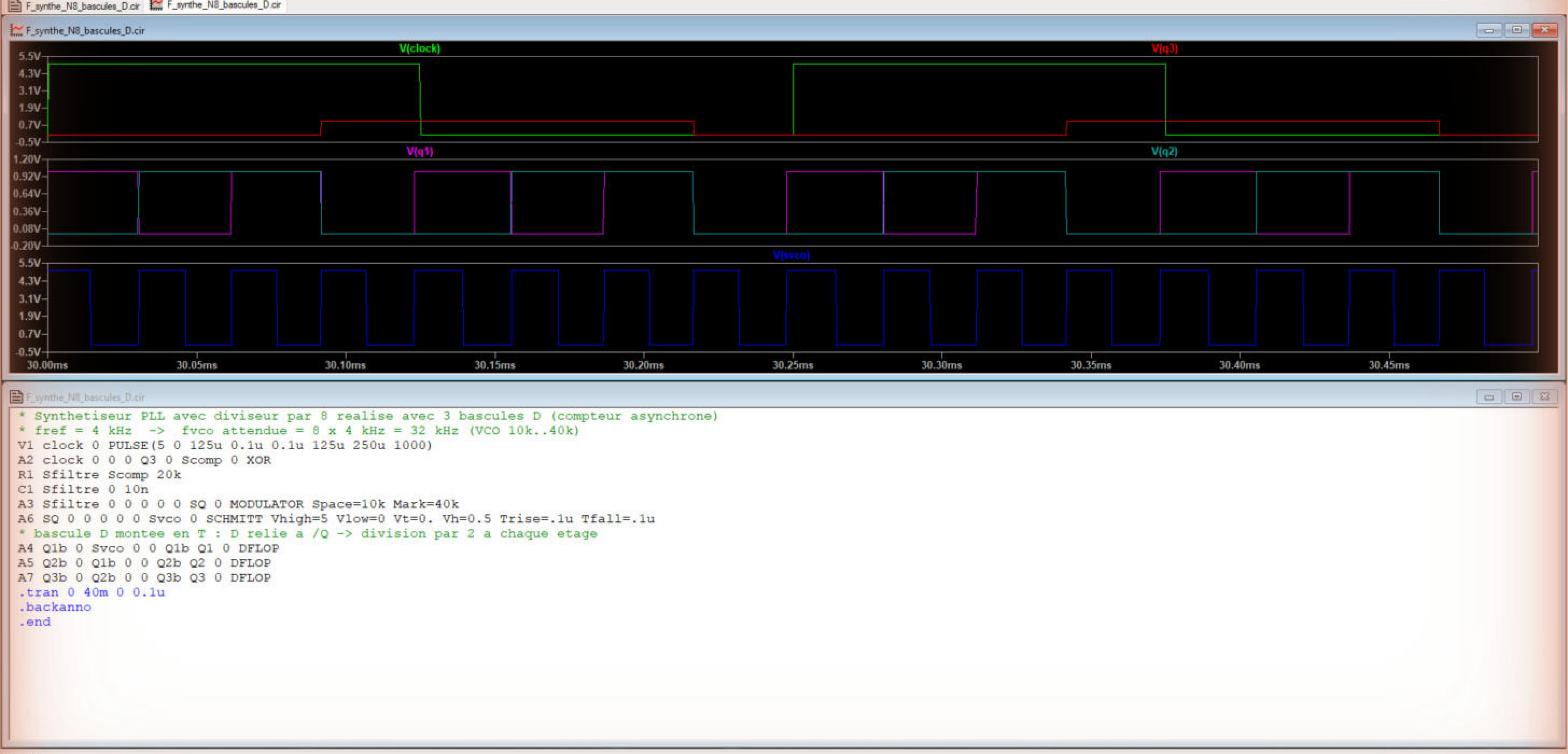
\includegraphics[width=\linewidth]{F25_N8_chronogrammes.png}
\caption{Diviseur par 8 : \texttt{clock} et \texttt{Q3} (4~kHz), \texttt{Q1} (16~kHz),
\texttt{Q2} (8~kHz) et \texttt{Svco} (32~kHz). La netlist est visible en bas.}
\label{fig:F25}
\end{figure}

\begin{figure}[H]
\centering
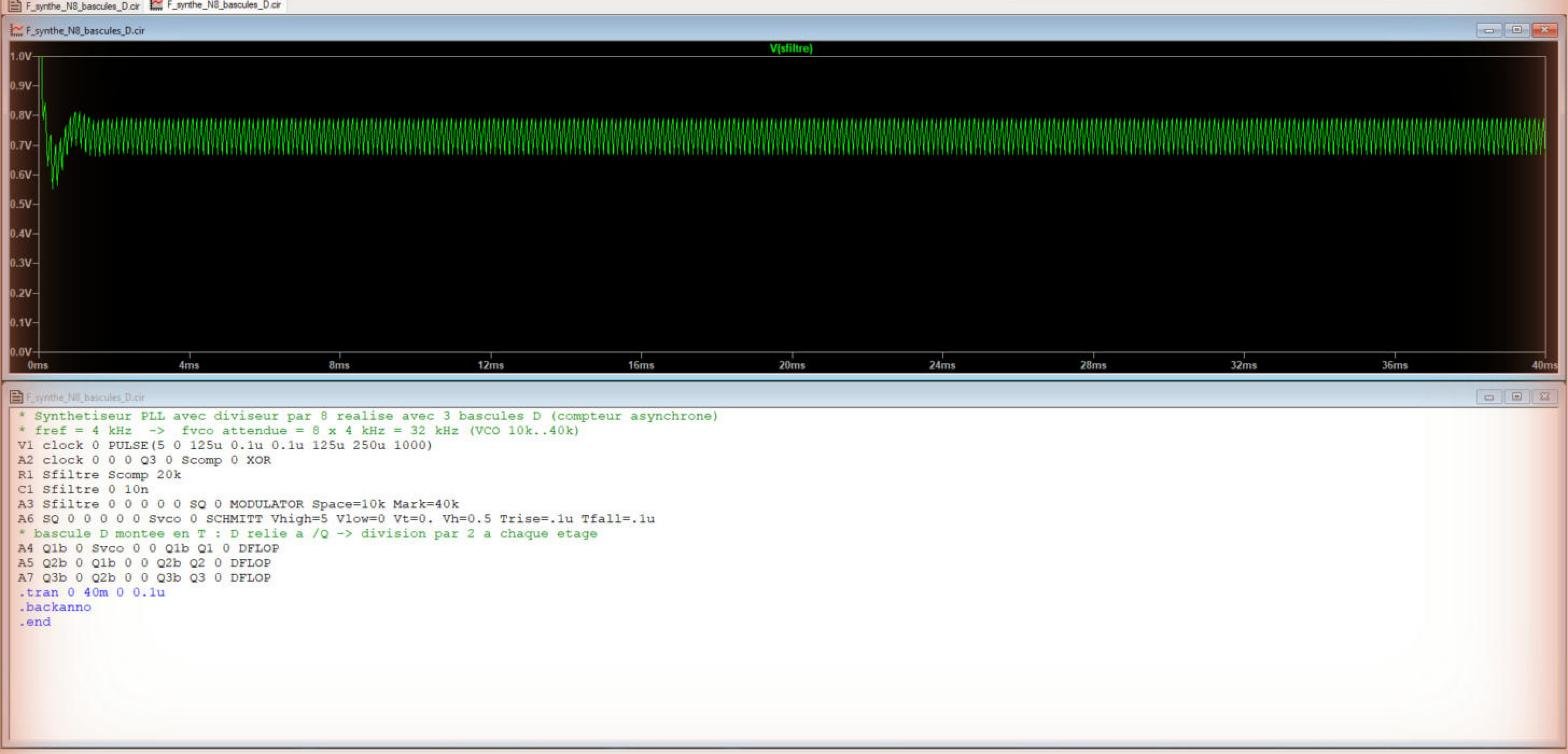
\includegraphics[width=\linewidth]{F25_N8_sfiltre.png}
\caption{Diviseur par 8 : tension \texttt{Sfiltre} sur 40~ms.}
\label{fig:F25s}
\end{figure}

Nous mesurons $f_{Q1} = 16{,}00$~kHz, $f_{Q3} = 4{,}000$~kHz $= f_{\text{clock}}$ et
$f_{\text{VCO}} = 32{,}00$~kHz. La valeur moyenne de \texttt{Sfiltre} vaut 0,733~V, et le temps
d'établissement est d'environ 1,2~ms. On compte bien huit périodes du VCO par période
d'horloge (figure~\ref{fig:F25}) : la synthèse $f_{\text{VCO}} = 8\,f_{\text{ref}}$ est vérifiée.

% ---------------------------------------------------------------------
\section{Conclusion (version complétée)}
Les simulations ont permis de vérifier chaque bloc de la PLL, puis de caractériser la boucle
complète. Avec un XOR de 0 à 1~V et un VCO de 0 à 40~kHz, la bande de verrouillage couvre
presque toute la plage du VCO (de 2,6 ou 6~kHz jusqu'à 39,8~kHz). La bande de capture dépend
en revanche fortement du filtre : 20,3~kHz avec 5~k$\Omega$ et seulement 5,8~kHz avec
50~k$\Omega$. Les échelons de fréquence montrent le compromis du filtre RC. Avec une résistance
faible, la boucle est rapide et sa capture est large, mais l'ondulation est forte. Avec une
résistance élevée, le filtrage est bon, mais la boucle est peu amortie, sa capture est étroite,
et elle ne s'accroche plus du tout à 80~k$\Omega$. En FSK, les sauts de fréquence doivent rester
dans la bande de capture (6~kHz au maximum avec 50~k$\Omega$). Enfin, le synthétiseur produit
exactement $N f_{\text{ref}}$ (30,006~kHz pour $N = 3$, 32,00~kHz pour $N = 8$) en environ 0,6 à 1,2~ms, mais l'ondulation du filtre crée des raies parasites à $\pm f_{\text{ref}}$
situées à environ $-16$~dB sous la porteuse. C'est la principale limite de ce montage simple.

\end{document}
